\scanpage{88}
Dans le cas où $\mathscr G$ est quelconque, on peut
définir cependant le \inserted{\unsure{lien|$L$}} $L'=\operatorname{corad}(L)$, qui est
commutatif, et il correspond à une
gerbe quotient $\mathscr G'$ de lien commutatif $L'$.
D'ailleurs, $L'$ correspond à un groupe
algébrique \inserted{$H$}, et ce qui précède prouve que
$(\operatorname{Ker}(\varepsilon:H\longrightarrow{}G_m))^{\unsure{\circ|0}}$ est un tore \uline{compact}.

\figure{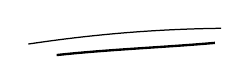
\begin{tikzpicture}
\draw[line width=.45pt] (0,0) .. controls (.8,.12) and (1.6,.19) .. (2.45,.20);
\draw[line width=.85pt] (.36,-.14) .. controls (1,-.07) and (1.75,-.04) .. (2.37,.015);
\end{tikzpicture}}

Nous envisageons maintenant une \deleted{gerbe}
catégorie de motifs munie d'un
\deleted{\unsure{automo|autre}} \unsure{hom|fonc|Frobenius} tensoriel dans \unsure{Abli-|Weil-|$\mathbb R$li-|Aut}$\unsure{\overline{\mathcal C}|\overline{=}}$
qui soit ``\unsure{génératrice|générateur}''. Ainsi $L$ est commutatif
et correspond à un groupe \deleted{\unsure{commutatif}}\inserted{\unsure{alg.}} \deleted{de type}
\deleted{\unsure{$G$}} multiplicatif $G$, \uline{muni} d'un
élément $f$ (``frobenius''), et $G$ est
engendré (au sens de Zariski) par
$f$. \deleted{Dans le cas qui nous occupe,}
\deleted{\unsure{Prenant le caractère|Prenant $L$ comme}\ \unsure{dessus}\unsure{,}}
\deleted{\unsure{soit|voit}}.
% archive sheet number: 87

